\chapter{Results} \label{Results}

\noindent The table below shows the 15 static and dynamic features used in our study for the purpose of gait recognition. We used a set of 5 classifiers: Linear SVM, Quadratic SVM, Fine KNN, Complex Trees and Neural Networks and we evaluate the performance of each classifier on the testing data in this section.
 

\def\arraystretch{1.28}
\begin{table}[h]
\centering
\begin{tabular}{| p{2cm} | |p{6cm}|}
 \hline
\cellcolor{pink} SR No. & \cellcolor{pink} Features  \\ \hline
1 & Height \\ \hline
2 & Length of full arms \\ \hline
3 & Length of fore arms \\\hline
4 & Length of upper arms \\ \hline
5 & Length of full legs \\ \hline
6 & Length of thighs \\\hline
7 & Length of lower legs \\\hline
8 & Distance between ankles  \\ \hline
9 & Distance between knees \\ \hline
10 & Distance between elbows  \\ \hline
11 & Distance between hands  \\ \hline
12 & Variance of head along X   \\ \hline
13 & Variance of head along Y  \\ \hline
14 & Variance of left knee along Y  \\ \hline
15 & Variance of right knee along Y  \\ \hline
\end{tabular}
\caption{ All the extracted features}
\end{table}


\noindent Before applying any classifier we normalized our feature matrix to the range [-1, 1]. Scaling data is very important in order to avoid attributes in greater numeric ranges dominating those in smaller numeric ranges. We also conducted a 3-fold cross-validation for the first four classifiers in order to evaluate the effectiveness of the proposed method. In a 3-fold cross-validation, the whole dataset is randomly divided into 3 subsets, where each subset contains an equal number of samples from each category. The classifier is trained on 2 subsets, while the remaining one is used for testing. The average classification rate is calculated after repeating the above process for 3 times.

\noindent In the case of Linear SVM, 14 gait samples of the testing set were classified correctly. Giving us an accuracy of 87.5\%. For the 2 samples which weren’t, one was misclassified and the other was not recognised by the classifier.

\noindent Quadratic SVM gave us the best accuracy of 93.75\% by categorizing 15 gait samples correctly. Surprising, the sample which was misclassified in Linear SVM was not recognised in this case.

\noindent Fine KNN yielded an accuracy of 81.25\%, 3 samples from the testing set were misclassified. On the other hand Complex Trees gave us the poorest success rate of 68.75\% were 2 samples were misclassified and 3 were not recognised by the classifier. 

\noindent In the case of neural networks, we set aside 10 \% data for validation and 5 \% for testing from the training database. Validation samples are used to measure network generalization, and to halt training when generalization stops improving, whereas testing samples have no effect on training and so provide an independent measure of network performance during and after training.\\



\newpage

\noindent The figure below shows the architecture of the network we implemented. It consists of 15 neurons in the input layer, one hidden layer with 12 neurons and the output layer with 9 neurons. The output layer has one neuron extra as compared to the number of classes, this is for the data that does not get recognised in the network.

\begin{figure}[h]
\centering
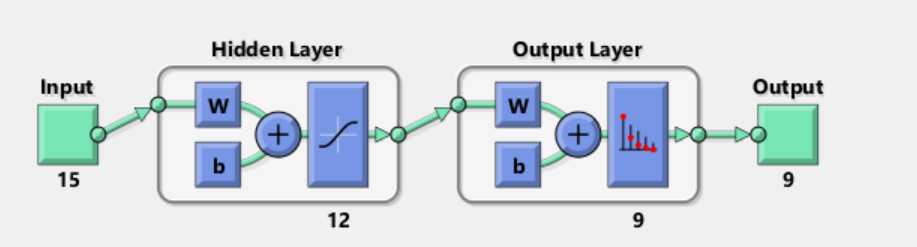
\includegraphics[scale=0.9]{anna.png}
\caption{ANN Architecture}
\end{figure}


\noindent When the output threshold was set at 0.9, neural network correctly identified 13 of the 16 samples in the testing database, accuracy of 81.25 \%. When this threshold was lowered to 0.8, the accuracy jumped to 93.75 \%, where the network not being able to identify just one sample.